%% Follow comments to support use.

%%%%%%%%%%%%%%%%%%%%%%%%%%%%%%%%%%%%%%%%%%%%%%%%%%%%%%%%%
%% STEP 1: Choose options for MSc / BSc / seminar layout and your bibliographic style
%%%%%%%%%%%%%%%%%%%%%%%%%%%%%%%%%%%%%%%%%%%%%%%%%%%%%%%%%

%%  Language: 
%%      finnish, swedish, or english
%%  Pagination (use twoside by default)  
%%      oneside or twoside,
%%  Study programme / kind of report
%%      csm  = Master's thesis in Computer Science Master's Programme;
%%      tkt = Bachelor's thesis in Computer Science Bachelor's Programme;
%%      seminar = seminar report
%%  For Master's thesis choose your line or track:
%%      (30 cr thesis, 2020 onwards, Master's Programme in Computer Science = csm)
%%      software-track-2020 = Software study track
%%      algorithms-track-2020 = Algorithms study track
%%      networking-track-2020 = Networking study track

\documentclass[english,twoside,censored,seminar,software-track-2020]{HYthesisML} 


% If wanted, open new chapters only at right page.
% By default, "openany".
%\PassOptionsToClass{openright,twoside,a4paper}{report}
\PassOptionsToClass{openany,twoside,a4paper}{report}

\usepackage{csquotes}
%%%%%%%%%%%%%%%%%%%%%%%%%%%%%%%%%%%%%%%%%%%%%%%%%%%%%%%%%
%% REFERENCES
%% Some notes on bibliography usage and options:
%% natbib -> you can use, e.g., \citep{} or \parencite{} for (Einstein, 1905); with APA \cite -> Einstein, 1905 without ()
%% maxcitenames=2 -> only 2 author names in text citations, if more -> et al. is used
%% maxbibnames=99 as no great need to suppress the biliography list in a thesis
%% for more information see biblatex package documentation, e.g., from https://ctan.org/pkg/biblatex 

%% Reference style: select one 
%% for APA = Harvard style = authoryear -> (Einstein, 1905) use:
\usepackage[style=authoryear,bibstyle=authoryear,backend=biber,natbib=true,maxnames=99,maxcitenames=2,uniquelist=minyear,giveninits=true,uniquename=mininit]{biblatex}
%% for numeric = Vancouver style -> [1] use:
%\usepackage[style=numeric,bibstyle=numeric,backend=biber,natbib=true,maxbibnames=99,giveninits=true,uniquename=init]{biblatex}
%% for alpahbetic -> [Ein05] use:
%\usepackage[style=alphabetic,bibstyle=alphabetic,backend=biber,natbib=true,maxbibnames=99,giveninits=true,uniquename=init]{biblatex}
%

\addbibresource{bibliography.bib}
% in case you want the final delimiter between authors & -> (Einstein & Zweistein, 1905) 
% \renewcommand{\finalnamedelim}{ \& }
% List the authors in the Bibilipgraphy as Lastname F, Familyname G,
\DeclareNameAlias{sortname}{family-given}
% remove the punctuation between author names in Bibliography 
%\renewcommand{\revsdnamepunct}{ }

% Asked chat.openai.com: I'm using biblatex package, but it prints odd format volume.number in reference list, while this should be volume (number). How to fix this?
%Answer (shortened):
% Redefine the volume and number format
%\DeclareFieldFormat[article]{volume}{\mkbibbold{#1}}
%\DeclareFieldFormat[article]{number}{\mkbibparens{#1}}
% Please remove the boldface from the volume and number fields:
\DeclareFieldFormat[article]{volume}{#1}
\DeclareFieldFormat[article]{number}{\mkbibparens{#1}}
% Now this generated format volume.(number). How to remove the dot? (and so on with some adjustments):
\renewbibmacro*{volume+number+eid}{%
  \setunit{\addcomma\space}% 
  \printfield{volume}%
  %\setunit*{\addnbspace\addthinspace}% <-- Adjust spacing here
  \printfield{number}%
  \setunit{\addcomma\space}%
  \printfield{eid}}


%% Block of definitions for fonts and packages for picture management.
%% In some systems, the figure packages may not be happy together.
%% Choose the ones you need.

%\usepackage[utf8]{inputenc} % For UTF8 support, in some systems. Use UTF8 when saving your file.

\usepackage{lmodern}         % Font package, again in some systems.
\usepackage{textcomp}        % Package for special symbols
\usepackage[pdftex]{color, graphicx} % For pdf output and jpg/png graphics
\usepackage{epsfig}
\usepackage{subfigure}
\usepackage[pdftex, plainpages=false]{hyperref} % For hyperlinks and pdf metadata
\usepackage{fancyhdr}        % For nicer page headers
\usepackage{tikz}            % For making vector graphics (hard to learn but powerful)
%\usepackage{wrapfig}        % For nice text-wrapping figures (use at own discretion)
\usepackage{amsmath, amssymb} % For better math

\singlespacing               %line spacing options; normally use single

\fussy
%\sloppy                      % sloppy and fussy commands can be used to avoid overlong text lines
% if you want to see which lines are too long or have too little stuff, comment out the following lines
% \overfullrule=1mm
% to see more info in the detailed log about under/overfull boxes...
% \showboxbreadth=50 
% \showboxdepth=50



%%%%%%%%%%%%%%%%%%%%%%%%%%%%%%%%%%%%%%%%%%%%%%%%%%%%%%%%%
%% STEP 2:
%%%%%%%%%%%%%%%%%%%%%%%%%%%%%%%%%%%%%%%%%%%%%%%%%%%%%%%%%
%% Set up personal information for the title page and the abstract form.
%% Replace parameters with your information.
\title{Set Intersection Problem}

\author{Marco Bellò}
\date{\today}

% Set supervisors, use the titles according to the thesis language
% in English Prof. or Dr., or in Finnish toht. or tri or FT, TkT, Ph.D. or in Swedish... 
\supervisors{Prof.~J.~Kärkkäinen, Prof.~V.~Mäkinen, Dr. ~D. ~Diaz}

\keywords{algorithms, data structures, set intersection, inverted index}
\additionalinformation{\translate{\track}}

%% For seminar reports:
\additionalinformation{Seminar in Algorithm Engineering}

%% Provide classification terms, to appear on the abstract page.
%% Replace the classification terms below with the ones that match your work.
%% ACM Digital library provides a taxonomy and a tool for classification
%% in computer science. Use 1-3 paths, and use right arrows between the
%% about three levels in the path; each path requires a new line.

\classification{\protect{\ \\
\  General and reference $\rightarrow$ Document types  $\rightarrow$ Surveys and overviews\  \\
\ Software and its engineering $\rightarrow$ Software creation and management $\rightarrow$ Designing software\ \\
\  Applied computing $\rightarrow$ Document management and text processing $\rightarrow$ Document searching\vspace*{1mm}
}}

%% If you want to quote someone special. You can comment this line out and there will be nothing on the document.
%\quoting{Bachelor's degrees make pretty good placemats if you get them laminated.}{Jeph Jacques}


%% OPTIONAL STEP: Set up properties and metadata for the pdf file that pdfLaTeX makes.
%% Your name, work title, and keywords are recommended.
\hypersetup{
    unicode=true,           % to show non-Latin characters in Acrobat’s bookmarks
    pdftoolbar=true,        % show Acrobat’s toolbar?
    pdfmenubar=true,        % show Acrobat’s menu?
    pdffitwindow=false,     % window fit to page when opened
    pdfstartview={FitH},    % fits the width of the page to the window
    pdftitle={Set Intersection},            % title
    pdfauthor={Marco Bellò},           % author
    pdfsubject={Set Intersection},          % subject of the document
    pdfcreator={},          % creator of the document
    pdfproducer={pdfLaTeX}, % producer of the document
    pdfkeywords={algorithms} {data structures} {set intersection} {inverted index}, % list of keywords for
    pdfnewwindow=true,      % links in new window
    colorlinks=true,        % false: boxed links; true: colored links
    linkcolor=black,        % color of internal links
    citecolor=black,        % color of links to bibliography
    filecolor=magenta,      % color of file links
    urlcolor=cyan           % color of external links
}

%%-----------------------------------------------------------------------------------
%%%%%%%%%%%%%%%%%%%%%%%%%%%%%%%%%%%%%%%%%%%%%%%%%%%%%%%%%%%%
% MY CUSTOM PACKAGES

\usepackage{wrapfig}

\usepackage{tabularx}

\usepackage{algpseudocode}

\usepackage{algorithm}

\newcommand\brref[1]{[\ref{#1}]} %make ref with brackets

%%%%%%%%%%%%%%%%%%%%%%%%%%%%%%%%%%%%%%%%%%%%%%%%%%%%%%%%%%%%%%

\begin{document}

% Generate title page.
\maketitle

%%%%%%%%%%%%%%%%%%%%%%%%%%%%%%%%%%%%%%%%%%%%%%%%%%%%%%%%%
%% STEP 3:
%%%%%%%%%%%%%%%%%%%%%%%%%%%%%%%%%%%%%%%%%%%%%%%%%%%%%%%%%
%% Write your abstract in the separate file, to be positioned here.
%% You can make several abstract pages (if you want it in different languages),
%% in which case you should also define the language of the abstract,
%% as below.

% \begin{abstract}{finnish}

% Tämä dokumentti on tarkoitettu Helsingin yliopiston tietojenkäsittelytieteen osaston opin\-näyt\-teiden ja harjoitustöiden ulkoasun ohjeeksi ja mallipohjaksi. Ohje soveltuu kanditutkielmiin, ohjelmistotuotantoprojekteihin, seminaareihin ja maisterintutkielmiin. Tämän ohjeen lisäksi on seurattava niitä ohjeita, jotka opastavat valitsemaan kuhunkin osioon tieteellisesti kiinnostavaa, syvällisesti pohdittua sisältöä.


% Työn aihe luokitellaan  
% ACM Computing Classification System (CCS) mukaisesti, 
% ks.\ \url{https://dl.acm.org/ccs}. 
% Käytä muutamaa termipolkua (1--3), jotka alkavat juuritermistä ja joissa polun tarkentuvat luokat erotetaan toisistaan oikealle osoittavalla nuolella.

% \end{abstract}

\begin{otherlanguage}{english}
\begin{abstract}
Write your abstract here.

In addition, make sure that all the entries in this form are completed.

Finally, specify 1--3 ACM Computing Classification System (CCS) topics, as per \url{https://dl.acm.org/ccs}.
Each topic is specified with one path, as shown in the example below, and elements of the path separated with an arrow.
Emphasis of each element individually can be indicated
by the use of bold face for high importance or italics for intermediate
level.

\end{abstract}
\end{otherlanguage}


% Place ToC
%\newpage
\mytableofcontents

\mainmatter

%%%%%%%%%%%%%%%%%%%%%%%%%%%%%%%%%%%%%%%%%%%%%%%%%%%%%%%%%
%% STEP 4: Write the thesis.
%%%%%%%%%%%%%%%%%%%%%%%%%%%%%%%%%%%%%%%%%%%%%%%%%%%%%%%%%
%% Your actual text starts here. You shouldn't mess with the code above the line except
%% to change the parameters. Removing the abstract and ToC commands will mess up stuff.
%%
%% Command \include{file} includes the file of name file.tex.
%% A new page will be created at every \include command, 
%% which makes it appropriate to use it for large entities such as book chapters. Cannot be nested.
%% It is useful for a big project, as changing one of the include targets 
%% won't force the regeneration of the outputs of all the rest.
%% Alternatively, \input is a more lower level macro 
%% which simply inputs the content of the given file like it was copy&pasted there manually.

\chapter{Introduction\label{intro}}

The act of "searching" has become so deeply ingrained in the modern society that we tend to take it for granted, not only assuming it normal to have immediate and easily accessible information on the tip of our thumbs, but expecting it: a study from 2004 showed that users were not willing to wait more than ten seconds for a page to load (\cite{waitTime}), fast forward twenty years and nowdays even a couple seconds holdup would be unacceptable, thus query retrieval needs to be fast. Blazingly fast in fact, since we need to account for all the delays typical of a gargantuan structure as big as the modern web, and, as the reader probably knows, it is \textit{not} a good idea to rely on memory's perfomances increasing over time: the smart way to tackle this problem is via research and development of efficient algorithms, and exactly which type should be self-evident from the title of this document. The problem of the set intersection constitutes the backbone of every query resolver in a (web) search engine, since every word in a query is interpreted as a collection of documents' IDs which contains it. \\
In this survey-style paper we will first explain what searching (i.e., querying) entails, show how a document (e.g., a web page) can be transformed into word tokens which are then further processed into inverted indexes, and, finally, we will see a collection of algorithms that concern themselves with intersecting sets, meaning finding common elements between two or more comparable collections. 

\subsection{How Do We Search?}

Generally speaking, a query is called a "bag of words", and finding its result means computing which documents contain all word tokens that are being searched for. Let's make and example: word \textit{abiura} is contained in documents number \textit{[31, 42, 127]}, while word \textit{bitonto} is contained in documents number \textit{20, 42, 72}. Thus \textit{query = (abiura,bitonto)} will return the result \textit{42}. \\
Both The example above and all the algorithms we will see in this survey consider the problem of searching as the problem of complete intersection, but modern search engine (e.g., Google)  leverage input relevance and filter unneeded outputs to obtain faster and better results, unfortunately finding information about how they do it is near impossible, since everything is covered by secrecy.
\chapter{Inverted Indexes\label{invindex}}

Most of the information present in this chapter is thanks to Mahapatra and Biswas "Inverted indexes: Types and techniques" \citep{fromDocToIndex}. 

What we will need for the algorithms presented in the rest of this documents are inverted indexes (also called posting lists). To get them we first need to process documents into lists of words (called \textit{word tokens}), then for each token compute a list of \verb+IDs+ that refer to the documents which contain that specific token. Let's see each step in order.

\section{Document Pre-Processing}

Documents go through a series of processing steps before being indexed: they get converted into token in the lexing phase, which are then possibly normalized, stemmed or even pruned (removed) entirely.

\subsection{Lexing}

\begin{wrapfigure}{r}{0.5\textwidth} %this figure will be at the right
    \centering
    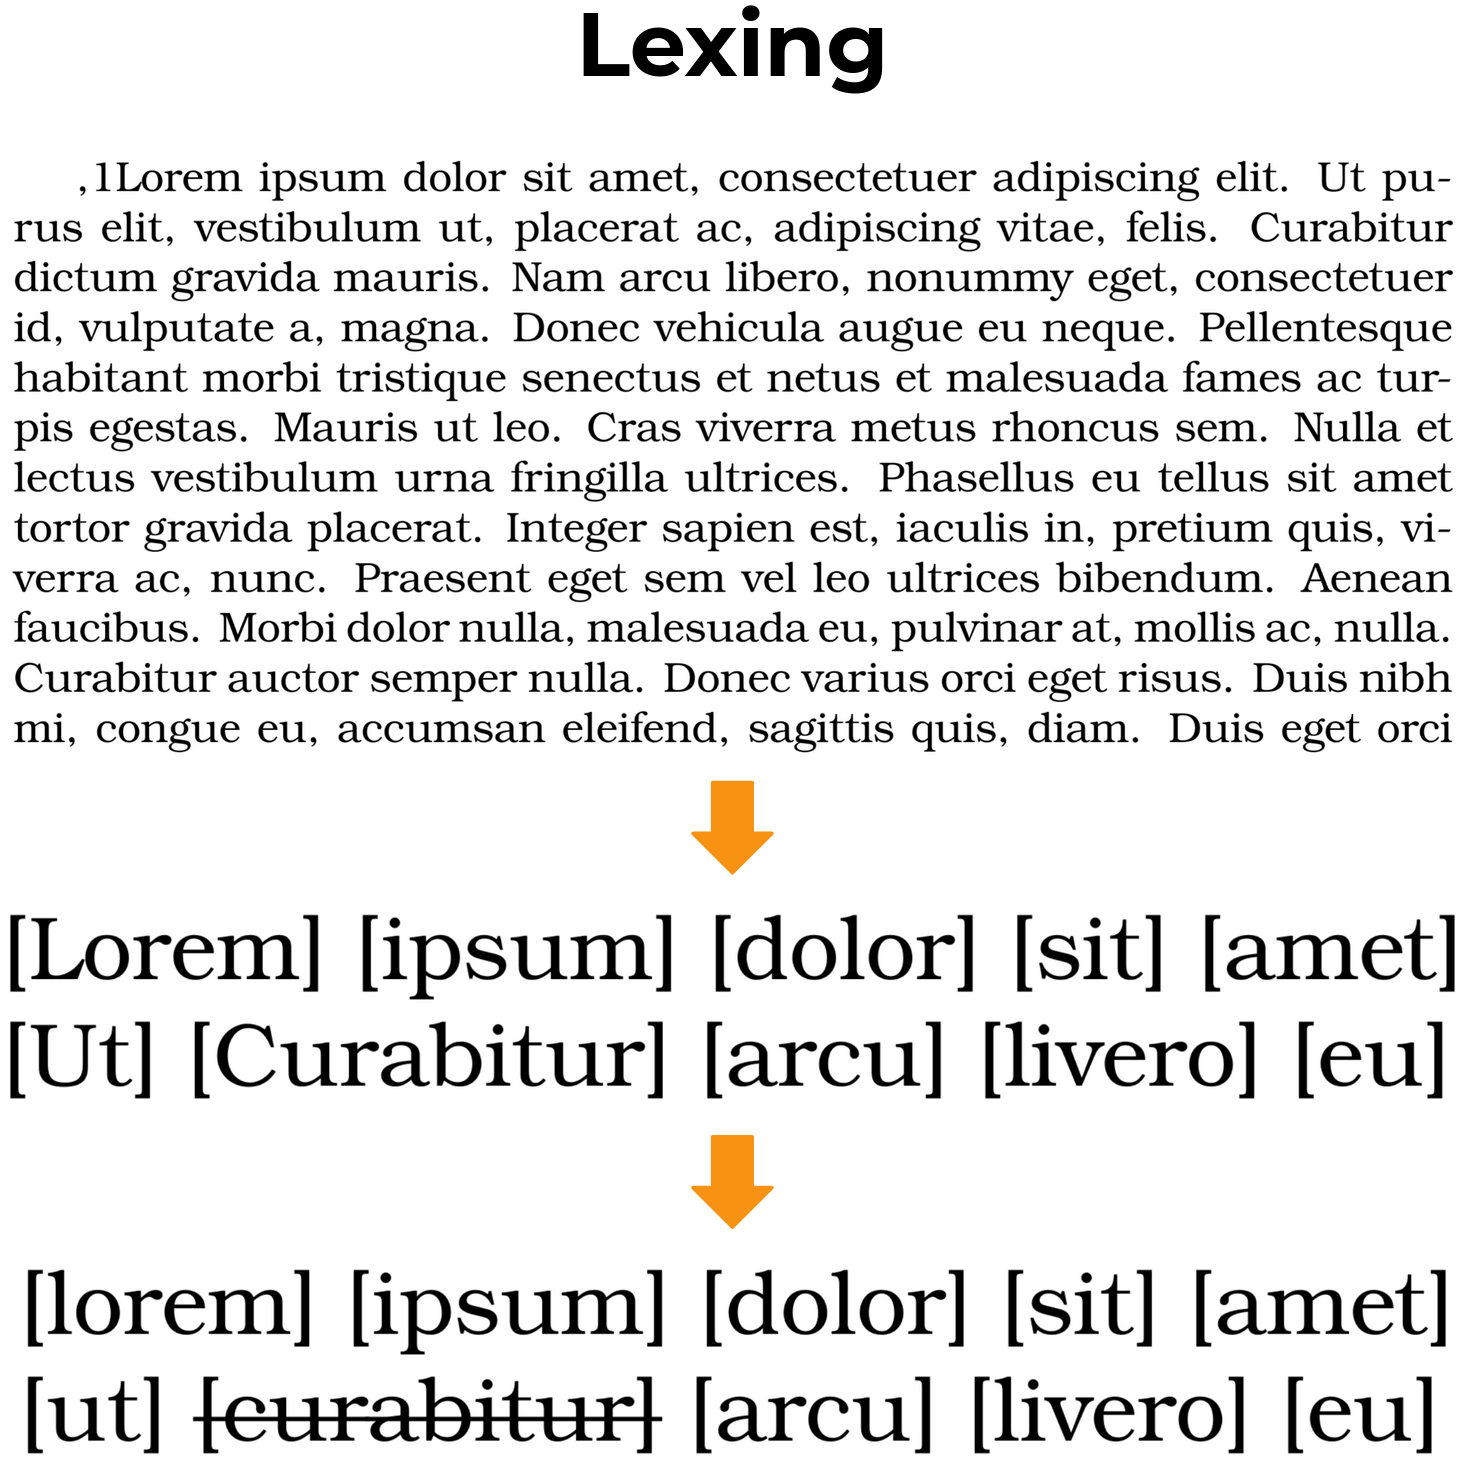
\includegraphics[width=.5\textwidth]{imgs/lorem_lexing.png}
    \caption{Lexing: from text to word tokens\label{fig:lorem_lexing}}
\end{wrapfigure}

The process of transforming a document into a list of tokens, each of which is a single word, si called \textit{lexing} \brref{fig:lorem_lexing}. There often is a maximum length for a single token, as to prevent unbounded index growth in edge cases, and all input is generally first converted into lower-case to normalize it. All non-punctuation characters are added to the list of tokens one by one, and those that exceed a certain size are often pruned (removed from the corpus). It is not entirely clear how Google and other big companies do this step, and it certainly feels strange to think they employ a simple \textit{brute force}, single scan approach, but as mentioned before it is not easy to find information about it. \\
All of the above works only with alphabetic languages, ideographic ones (e.g., Chinese) need specialized search techniques. 

\subsection{Stemming}

We can consider this step deprecated, since nowadays memory, especially for things like text and arrays (which inverted index basically are), is cheap and bountiful. \\
The idea is to find a sort of \textit{root} (stem) of the words, and indexing that instead. To make an example: fishnet, fishery, fishing, fishy, fishmonger, can all be boiled down to their stem \textit{fish} \brref{fig:fishstem}. 

\begin{figure}[ht] 
\begin{center}
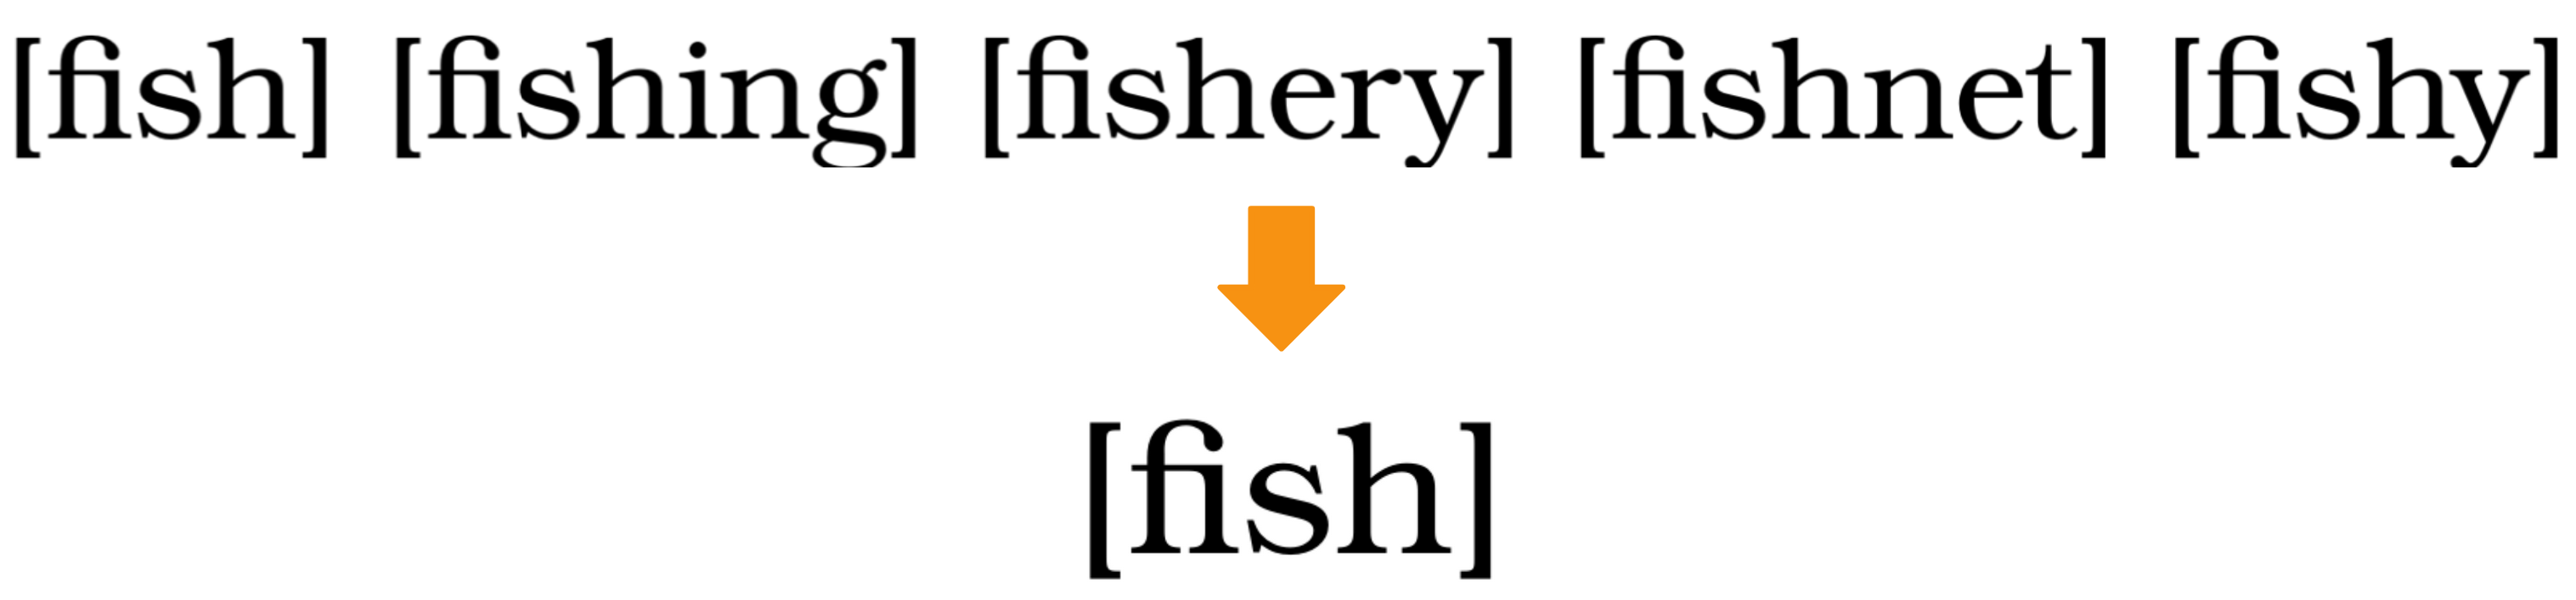
\includegraphics[width=.8\textwidth]{imgs/stemming.png}
\caption{Stemming to stem "fish"\label{fig:fishstem}}
\end{center}
\end{figure}

In the example above should be clear already that stemming carry some problems: a user searching for "fishnet" is likely not shopping for fishing equipment, thus most modern search engine skip this normalizing step, and most stemming algorithms (most famous of which is Porter's) are complex, full of exceptions and exceptions to the exceptions, while still failing to unite together the correct words. This step basically reduces query precision while providing very little in return.

\subsection{Stop Words}

\textit{Stop words} are words that work as connectives of sorts, like \textit{and}, \textit{the}, \textit{is}, \textit{of}, \textit{to}, etc. \\
Their quantity is language dependent (e.g., in English they could be around 500 words) and they are often removed from the corpus which, for normal queries, does not worsen the results while saving space in the index. However in some cases like searching for \textit{to be or not to be} stop words are actually essential, and removing them would make the search fail. \\ 

\begin{wrapfigure}{r}{0.5\textwidth} %this figure will be at the right
    \centering
    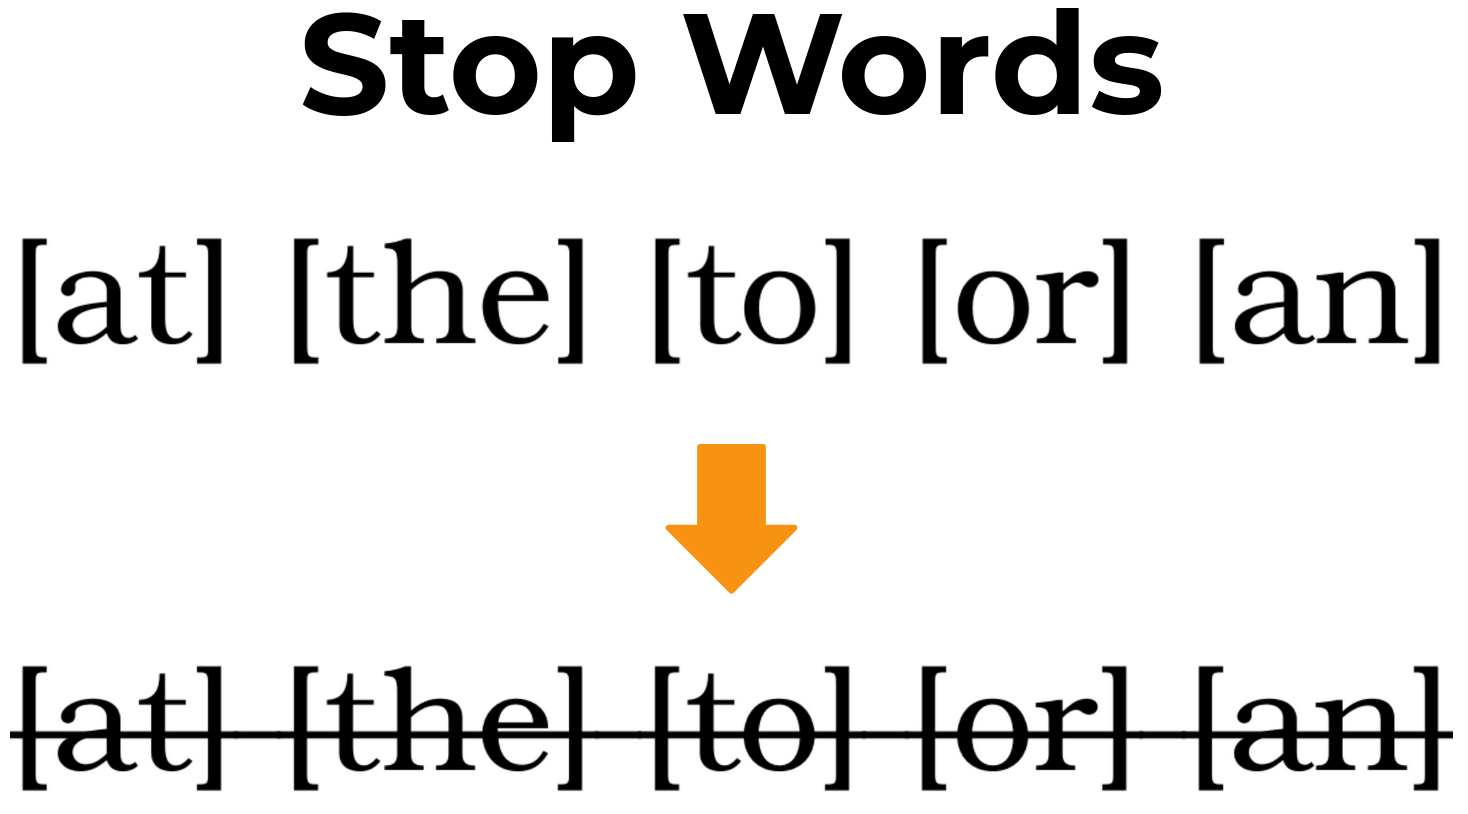
\includegraphics[width=.4\textwidth]{imgs/stopwords.png}
    \caption{Stop words pruning\label{fig:stopwords}}
\end{wrapfigure}

Thankfully they are so common that if saved as differences between consecutive different values, both their document number and word position lists can be compressed to save space. Because of this, the overhead is not as big as one might think, thus modern search engines (like Google) do not seem to remove them from the index, since doing so put them at a competitive advantage at the expense of a slightly bigger index. \\ 

\section{Inverted Indexes}

Now that we have a set of word tokens, we can start building our inverted indexes (or posting lists): documents are often stored as lists of words, but we invert (hence the name) this concept by storing for each word the list of documents that contain it. There are several variants of this data structure, but at minimum you need to store for each word the list of documents that contain that specific word. \\
We can change the granularity by adding the frequency of the word in the document, which can be useful for query optimization, or by adding the word position in the document, allowing for in-document queries.\\
Space used by inverted indexes varies wildly in the range of five to one hundred percent (5-100\%) of the total size of the document indexed, and this is because implementations come in many different variations: some store word positions and some don't, some aggressively pre-process documents and some don't, some dynamically update themselves and some don't, some use complex and powerful compression methods and some don't, and so on. 

Table \brref{tab:sample_docs} show some sample documents, while table \brref{tab:inverted_lists} shows some examples of inverted indexes, with different levels of granularity.

\begin{table}[ht]
    \begin{center}
        \begin{tabularx}{\textwidth}{|c|X|}
            \hline
            \textbf{ID} & \multicolumn{1}{c|}{\textbf{Contents}}  \\ \hline
            1 & The only way not to think about money is to have a great deal of it \\ \hline
            2 & When I was young I thought that money was the most important thing in life; now that I am old I know that it is. \\ \hline
            3 & A man is usually more careful of money than he is of his principles.\\ \hline
        \end{tabularx}
        \caption{Sample document collection\label{tab:sample_docs}}
    \end{center}
\end{table}

\begin{table}[ht]
    \begin{center}
        \begin{tabular}{|c|c|c|c|}
            \hline
            \textbf{Word} & \textbf{Doc List} & \textbf{Frequency} & \textbf{Positions} \\ \hline
            a & 1, 3 & 1:1, 3:1 & 1:(12), 3:(1) \\ \hline
            About & 1 & 1:1 & 1:(7) \\ \hline
            am & 2 & 2:1 & 2:(19) \\ \hline
            Careful & 3 & 3:1 & 3:(6) \\ \hline
            deal & 1 & 1:1 & 1:(16) \\ \hline
            great & 1 & 1:1 & 1:(13) \\ \hline
            have & 1 & 1:1 & 1:(11) \\ \hline
            ... & ... & ... & ... \\ \hline
            money & 1, 2, 3 & 1:2, 2:1, 3:1 & 1:(8), 2:(8), 3:(9) \\ \hline
            more & 3 & 3:1 & 3:(5) \\ \hline
            ... & ... & ... & ... \\ \hline
            when & 2 & 2:1 & 2:(1) \\ \hline
        \end{tabular}
        \caption{Inverted lists example, most words omitted\label{tab:inverted_lists}} 
    \end{center}
\end{table}



\chapter{Intersection Algorithms\label{intersect}}

In this chapter we are going to see a collection of algorithms to compute the intersection of two \textbf{sorted} lists, taken from the chapter six of "Pearl of Algorithm Engineering" by Paolo Ferragina, published by Cambridge University Press \citep{Ferragina_2023}. \\
We will first look at two of the most commonly used search algorithms, since we cannot intersect without searching. \\

\section{Search Algorithms}

\subsection{Binary Search \label{sec:binsearch}}

\begin{figure}[H] 
    \begin{center}
        \includegraphics[width=.8\textwidth]{imgs/Binary_Search_Depiction.png}
        \caption{Binary search algorithm, source: \href{https://en.wikipedia.org/wiki/Binary_search}{Wikipedia}\label{fig:binsearch}}
    \end{center}
\end{figure}

Binary search, also known as logarithmic search or binary chop, is a search algorithm that finds the position of a target value within a sorted array: it compares the target to the middle element of the array and, if they are not equal, it eliminates half of the search space by discarding either the left or right half, depending on whether the target value is less than or greater than the middle element. This process is repeated by iteratively searching into the remaining sub-array until the target value is found or the search space is empty. The pseudocode for the algorithm can be seen at \textit{Algorothm} \brref{alg:binsearch}.\\
Binary search runs in logarithmic time in the worst case, doing $O(\log n)$ comparisons, where $n$ is the number of elements in the array, making it much faster than linear search with large arrays thanks to its scaling.\\

\begin{algorithm}
    \captionsetup{labelsep=newline}
    \caption{Pseudocode for binary search algorithm \label{alg:binsearch}}
    \begin{algorithmic}[1]
        \State looking for element $key$
        \State let $L=0$ \Comment{First half}
        \State let $R=n-1$ \Comment{Second half}
        \While{$L\leq R$}
            \State $m=\lfloor (L+R)/2 \rfloor$
            \If{$A[M] < key$}
                \State let $L=m+1$
            \ElsIf{$A[M] > key$}
                \State $R = m - 1$
            \Else
                \State \Return $m$ \Comment{Found}
            \EndIf
        \EndWhile
        \State \Return false \Comment{Not found}
    \end{algorithmic}
\end{algorithm}

\subsection{Exponential Search}

\begin{figure}[H] 
    \begin{center}
        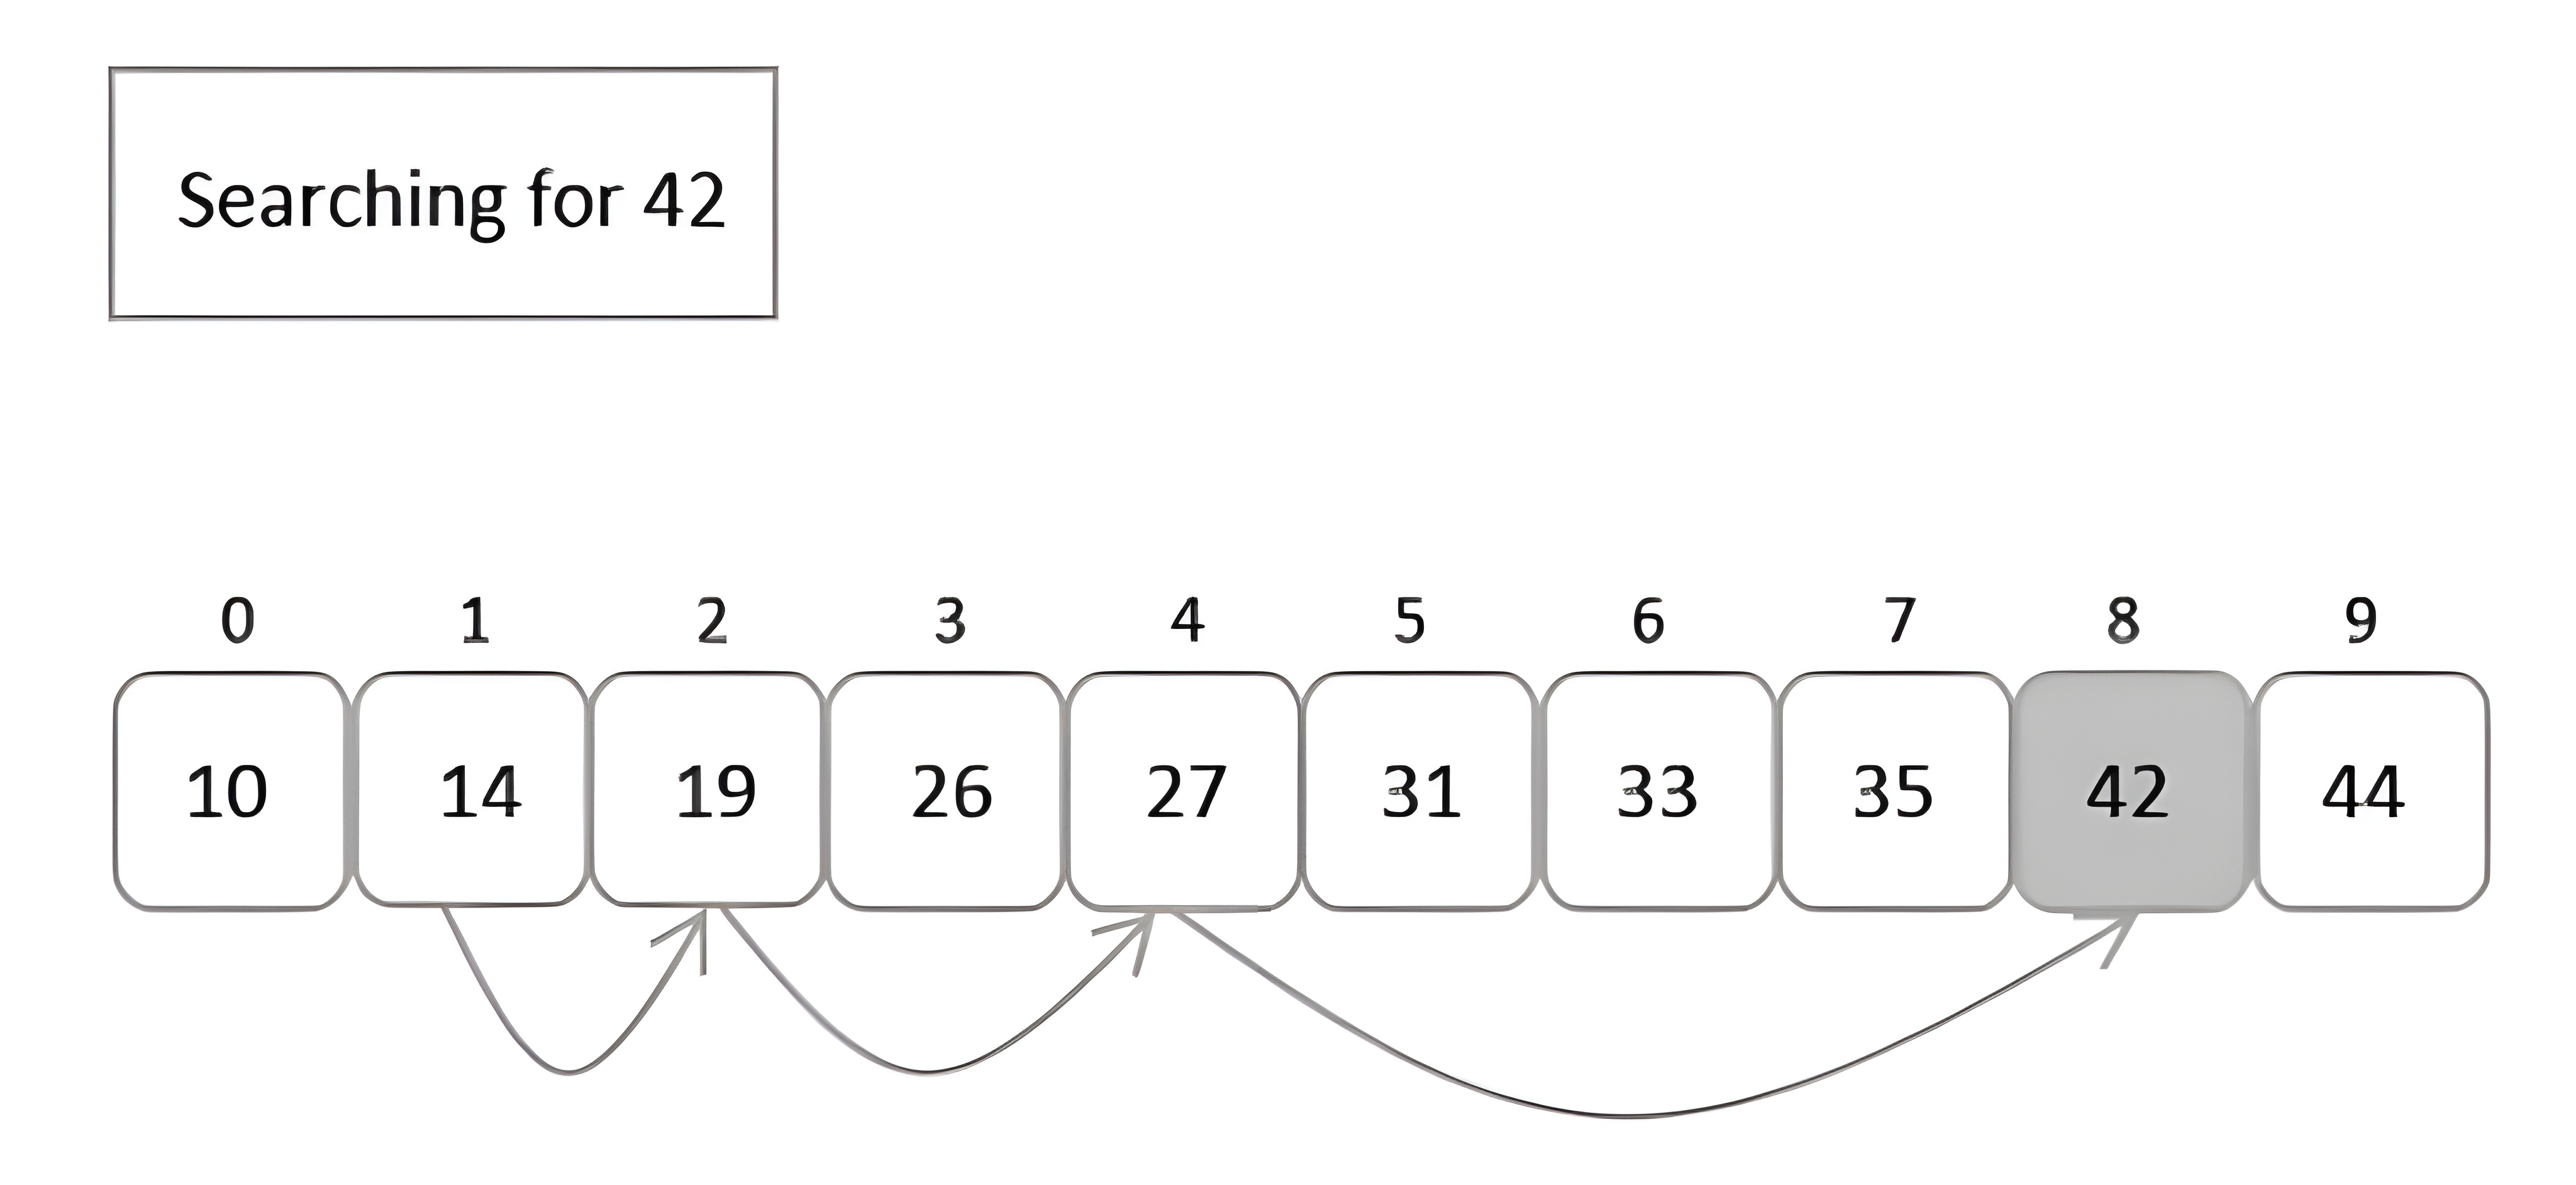
\includegraphics[width=.8\textwidth]{imgs/exponential_search.png}
        \caption{Exponential search algorithm, source: \href{https://www.tutorialspoint.com/data_structures_algorithms/exponential_search.htm}{Tutorialspoint}\label{fig:expsearch}}
    \end{center}
\end{figure}

Exponential search, also called doubling or galloping search, is an algorithm for searching sorted, unbounded lists: there are numerous implementations, most common being determining a sub-array into which the \verb|key| may resides in and performing a binary search \brref{sec:binsearch} within its range.\\
To be more precise: we go trough the list in exponentially increasing steps, with a factor of $2^k$ such that we first look into \verb+list[0]+, then \verb+list[1]+, then \verb+list[2]+, \verb+list[4]+, \verb+list[8]+, following with \textit{16}, \textit{32}, \textit{64}, \textit{128} and so on until we find a value that is greater than the \verb|key|. Once we find it, we perform a binary search between the previous jump and the current (or the end of the array): $2^{k-1} \leq key \leq min(2^{k},n)$.

The algorithm can be more efficient than binary search, as it runs in $O(\log i)$ time, where $i$ is the index of the element being searched for, which could be half if not less than $n$.\\
The pseudocode can be seen at \textit{Algorithm} \brref{alg:expsearch}.\\

\begin{algorithm}
    \captionsetup{labelsep=newline}
    \caption{Pseudocode for exponential search algorithm \label{alg:expsearch}}
    \begin{algorithmic}[1]
        \State looking for element $key$
        \State let $i=0$ 
        \State let $k=0$
        \While{($key>list[i+2^k]$ and $i<n$)} 
            \State $i=i+2^k$ \Comment Gallop to next step
            \State $k=k+1$ \Comment Increment exponent
        \EndWhile
        \If{$i<n$}
            \State binary\_search($list$, $key$, $i$, $min(i+2^k,n)$) 
        \Else
            \State \Return false \Comment{Not found}
        \EndIf
    \end{algorithmic}
\end{algorithm}

\subsection{Extrapolation and Intrapolation \label{sec:extrapol}}

TODO maye or maybe not 

\section{Intersection Algorithms}

\subsection{Brute Force \label{sec:bruteforce}}

The first idea that would come to mind when thinking about intersecting two lists is to simply iterate through both of them and check if the elements are equal: this is the \textit{brute force} approach, which is simple but inefficient. \\
With a time complexity of $O(m \cdot n)$, assuming lists sizes $n$ and $m$ to be around $10^6$, and assuming a modern computer able to do $10^9$ operations per second, this algorithm would need ten minutes to compute a 2-words query, which is less than ideal.\\
The (very short) pseudocode can be seen at \textit{Algorithm} \brref{alg:bruteforce}.\\

\begin{algorithm}
    \captionsetup{labelsep=newline}
    \caption{Pseudocode for brute force algorithm \label{alg:bruteforce}}
    \begin{algorithmic}[1]
        \ForAll{$i=0$ to $n-1$}
            \ForAll{$j=0$ to $m-1$}
                \If{$A[i] == B[j]$}
                    \State add $A[i]$ to result
                \EndIf
            \EndFor
        \EndFor
    \end{algorithmic}
\end{algorithm}

\subsection{Bunny Race}

\begin{figure}[H] 
    \begin{center}
        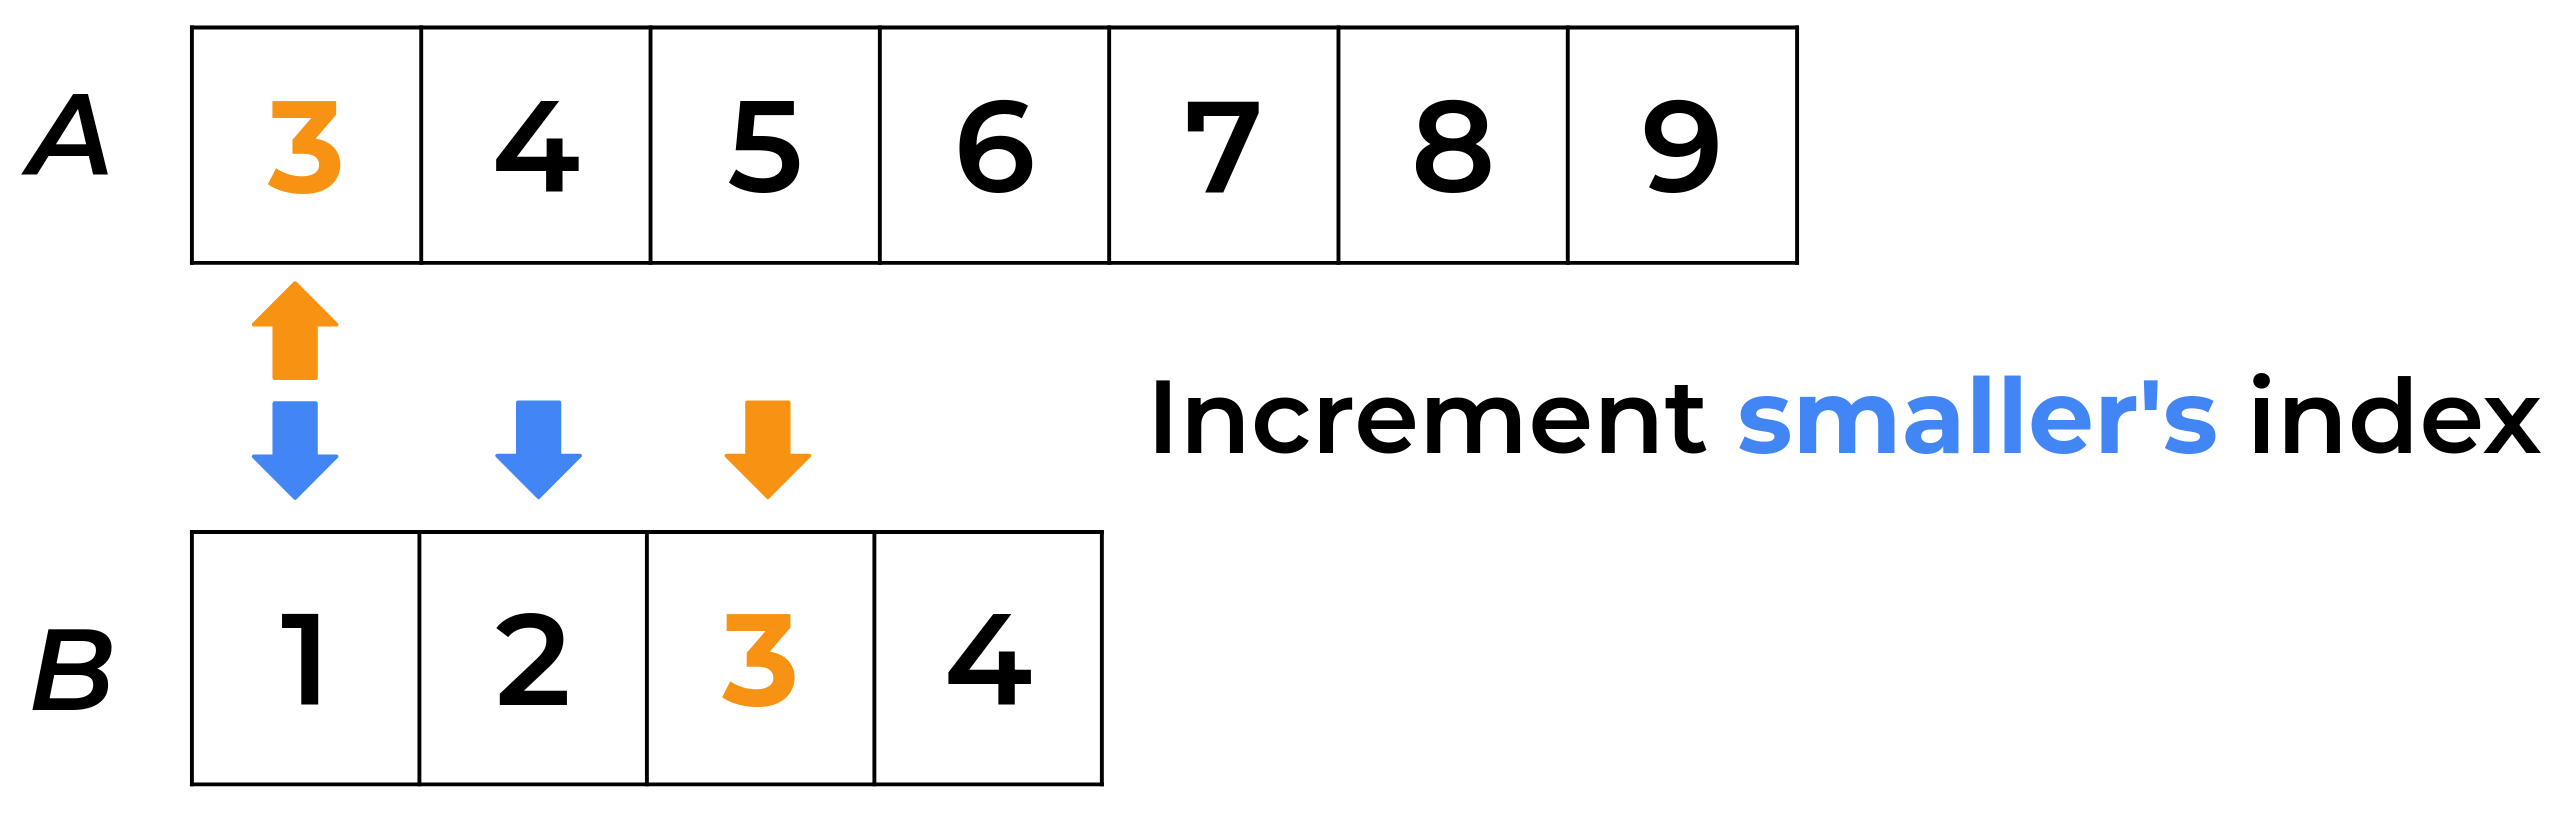
\includegraphics[width=.8\textwidth]{imgs/bunny_search.png}
        \caption{Bunny race algorithm \label{fig:bunnyrace}}
    \end{center}
\end{figure}

This approach, often called merge-based, is simple, elegant and fast: the main idea is to have two indices pointing at the two list running after each other by comparing elements each time and incrementing the index pointing at the smallest one (or incrementing both if they are equal).\\ 
To clarify: lets say we have two lists, $A$ and $B$, of size $n$ and $m$ respectively. We start with two pointers, $i$ and $j$, both set to zero. \\
We compare the elements at these indices, $A[i]$ and $B[j]$: if they are equal, we add the element to the result and increment both pointers. \\
If $A[i] < B[j]$, we increment $i$, while if $A[i] > B[j]$, we increment $j$. \\
This process continues until one of the pointers reaches the end of its respective list.\\
The correctness can be proven inductively, exploiting the following observation: if $A[i] < B[j]$ then $A[i]$ is smaller than all elements following $B[j]$ in $B$ since its ordered, so $A[i] \notin B$. The other case is symmetric. \\
In regards to time complexity, we just need to note that at each step the algorithm executes one comparison and advances at least one iterator, thus, given that $n=|A|$ and $m=|B|$, the algorithm runs in no more than $O(n+m)$ time.\\
This time complexity is significantly better than the \textit{brute force} \brref{alg:bruteforce} approach, since it can compute a 2-word query in $10^{-3}$ seconds. \\
The pseudocode can be seen at \textit{Algorithm} \brref{alg:bunnyrace}.

In the case that $n=\Theta (m)$ this algorithm is optimal, because we need to process the smallest set, thus $\Omega(min(n,m))$ is an obvious lower bound. Moreover, this procedure is also optimal in the disk model since it takes $O(\frac{n}{B})$ I/Os. \\
In the case that $n \ll m$ the classic \textit{binary search} can be helpful since we can design an algorithm that search in $A$ for each elements of $B$ in $O(m \log n)$ time, which is better than $O(n+m)$ when $m=o(\frac{n}{\log n})$.

\begin{algorithm}
    \captionsetup{labelsep=newline}
    \caption{Pseudocode for bunny race algorithm \label{alg:bunnyrace}}
    \begin{algorithmic}[1]
        \State let $i=0$ 
        \State let $j=0$ 
        \While{$i<n$ and $j<m$}
            \If{$A[i] < B[j]$}
                \State $i=i+1$ \Comment Increment first
            \ElsIf{$A[i] > B[j]$}
                \State $j=j+1$ \Comment Increment second
            \Else
                \State add $A[i]$ to result \Comment Found
                \State $i=i+1$  \Comment Increment both
                \State $j=j+1$
            \EndIf
        \EndWhile
    \end{algorithmic}
\end{algorithm}

\subsection{Divide and Search}

\begin{figure}[H] 
    \begin{center}
        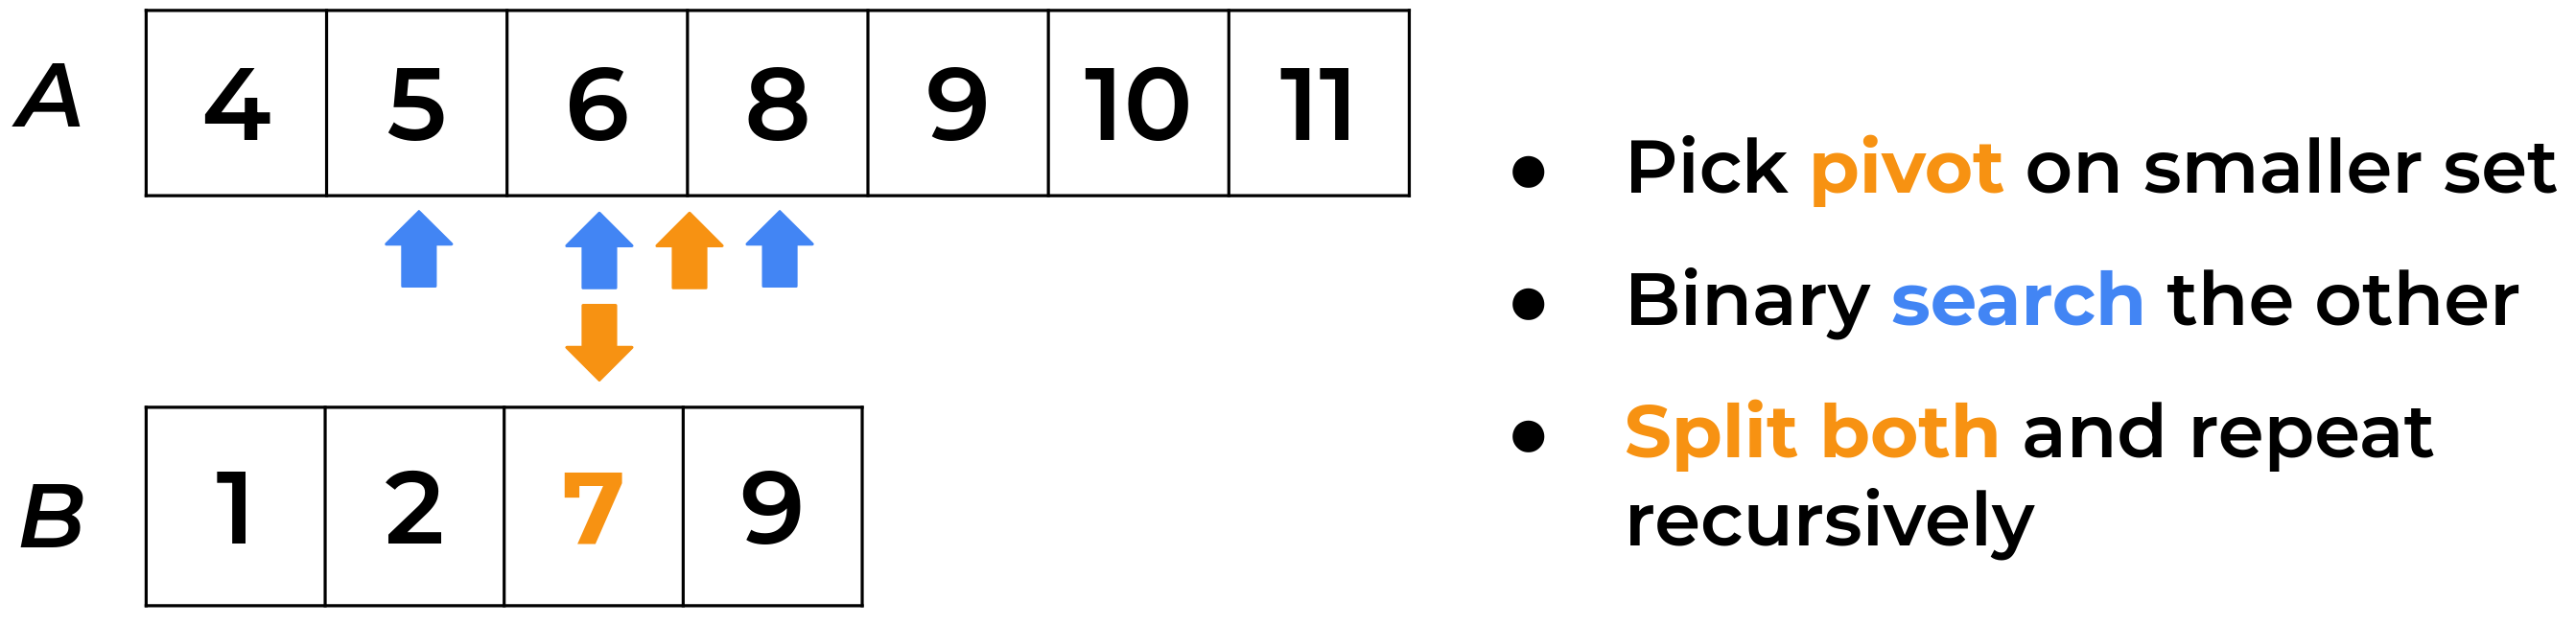
\includegraphics[width=.8\textwidth]{imgs/divide_and_search.png}
        \caption{Divide and search algorithm \label{fig:divandsearch}}
    \end{center}
\end{figure}

Also called \textit{mutual partitioning}, this approach adopt a classic algorithmic paradigm, namely \textit{divide and conquer}, famously used to design the \textit{quick sort} algorithm (which can be visualized \href{https://en.wikipedia.org/wiki/Quicksort}{here}).\\
Let us assume $m=|B| \leq n=|A|$. We select the median element of $B$, $b_{m/2}$, as a \textit{pivot} and search for it in the longer sequence $A$ using the \textit{binary search} \brref{sec:binsearch} algorithm.\\
Two cases may occur: 

\begin{itemize}
    \item[i.] \textit{pivot} is one of the elements fo the intersection;
    \item[ii.] $b_{m/2} \notin A$, e.g, $A[j]<b_{m/2}<A[j+1]$.
\end{itemize}

In both cases the algorithm proceeds \textit{recursively} by calling itself on the two sub-lists in which each list ($A$ and $B$) has been split according to the \textit{pivot} element, thus computing the following intersections:

\begin{itemize}
    \item $A[1, j] \cap B[1, m/2-1]$
    \item $A[ j+1, n] \cap B[m/2+1, m]$.
\end{itemize}

In simpler terms: we pick the middle element of the smaller list, search for it in the bigger list, split both lists and repeat the process recursively on the remaining sub-lists, then again, then again, then again, until we reach the base case where each list is of size one.\\
The pseudocode of the algorithm can be seen at \textit{Algorithm} \brref{alg:divandsearch}.\\

Correctness follows, while for evaluating time complexity we need to identify the worst case. \\
Let us start with the case where \textit{pivot} falls outside \textit{A}, meaning that one of the two parts is empty and thus the corresponding half of \textit{B} can be ignored. So, one \textit{binary search} \brref{sec:binsearch} over \textit{A}, costing $O(\log n)$ time, has discarded half of \textit{B}.\\
If this keeps occurring in all recursive calls, the total number of them will be $O(\log m)$, which leads us to a time complexity of $O(\log m \log n)$.\\
On the other hand, if we have both balanced partitions so that $b_{m/2}$ not only falls inside \textit{A} but coincides with the median element $a_{n/2}$, the time complexity can be expressed via the recurrence relation $T(n, m) = O(\log n) + 2T(\frac{n}{2}, \frac{m}{2})$, with the base case $T(n,m)=O(1)$ whenever $n,m \leq 1$.\\
This recurrence has the solution $T(n,m)=O(m(1+\log \frac{n}{m})) \forall m \leq n$, which is an optimal time complexity in the comparison model.

\begin{algorithm}
    \captionsetup{labelsep=newline}
    \caption{Pseudocode for divide and search algorithm \label{alg:divandsearch}}
    \begin{algorithmic}[1]
        \State Let $m=|B| \leq n=|A|$
        \State Pick \textit{pivot} $p=b_{\lfloor m/2 \rfloor}$
        \State \textit{Binary search} for \textit{p} in \textit{A} \Comment Say $a_j \leq p < a_{j+1}$
        \State \textit{Divide and search} on $A[1, j] \cap B[1, m/2 - 1]$
        \If{$p=a_j$}
            \State Add \textit{p} to result
        \EndIf
        \State \textit{Divide and search} on $A[ j + 1, n] \cap B[m/2 + 1, m]$
    \end{algorithmic}
\end{algorithm}
%\chapter{Discussion\label{discussion}}

\chapter{Conclusions\label{conclusions}}


%%%%%%%%%%%%%%%%%%%%%%%%%%%%%%%%%%%%%%%%%%%%%%%%%%%%%%%%%
%\cleardoublepage                          %fixes the position of bibliography in bookmarks
%\phantomsection
\addcontentsline{toc}{chapter}{\bibname}  % This lines adds the bibliography to the ToC
\printbibliography

%%%%%%%%%%%%%%%%%%%%%%%%%%%%%%%%%%%%%%%%%%%%%%%%%%%%%%%%%
%%%%%%%%%%%%%%%%%%%%%%%%%%%%%%%%%%%%%%%%%%%%%%%%%%%%%%%%%

\end{document}
